\begin{frame}
\frametitle{$\photon+\text{jet}$ events: jet calibration, balancing method}
\manip The physics of the events gives
\begin{equation*}
\vpT^\photon_\ptcl + \vpT^\text{jet}_\ptcl = \vec{0} \Rightarrow \boxed{{\pT}^\photon_\ptcl = {\pT}^\text{jet}_\ptcl}
\end{equation*}

\pause
\vfill

\manip For the reconstructed objects, the balancing response is then defined as
\begin{equation*}
\vpT^\photon_\reco + \underbrace{\Rbal \vpT^\text{jet}_\ptcl}_{\vpT^\text{jet}_\reco} = \vec{0}
\Rightarrow
\boxed{\Rbal = \frac{{\pT}^\text{jet}_\reco}{\pT^\photon}}
\end{equation*}
\begin{equation*}
\text{because }
\pT^\photon_\ptcl\simeq\pT^\photon_\reco
=\pT^\photon
\mend
\end{equation*}
\end{frame}

\begin{frame}
\frametitle{$\photon+\text{jet}$ events: world is not perfect}
\begin{center}
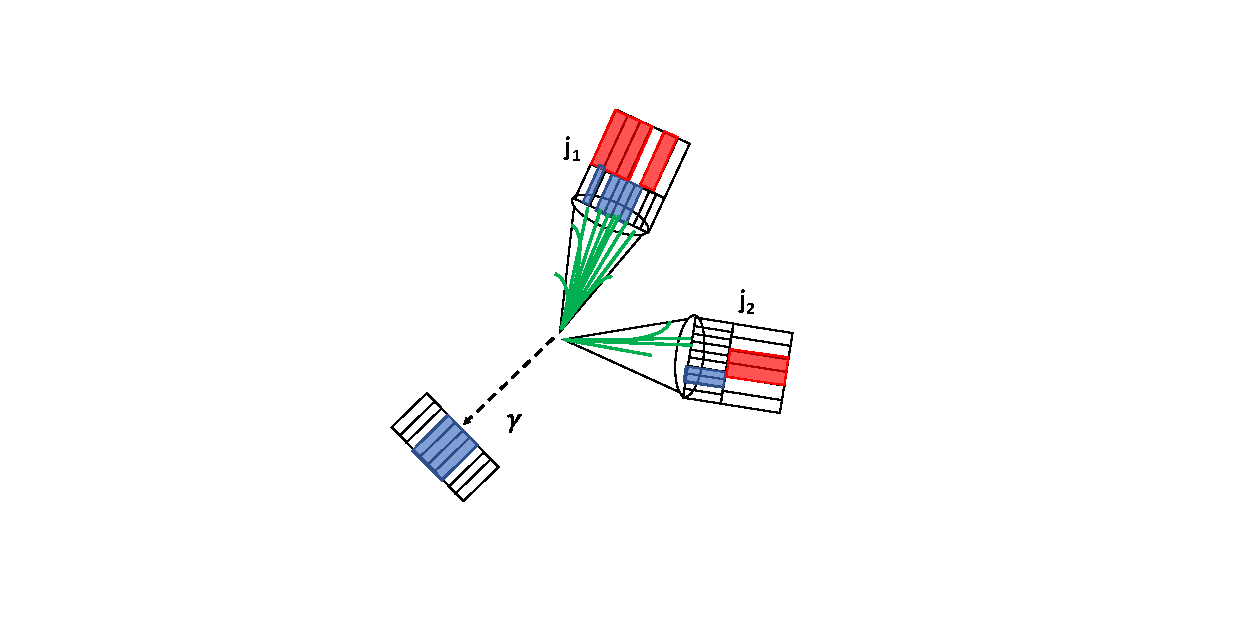
\includegraphics[width=\graphw,height=\graphh,keepaspectratio, trim = 5.5cm 2cm 7.5cm 1.75cm, clip]{\PhDthesisdir/tex/slides/JERC/JEC_Principe/Gamma_plus_two_jets.pdf}
\end{center}
\end{frame}

\begin{frame}
\frametitle{$\photon+\text{jet}$ events: world is not perfect}
\manip Imbalance due to the presence of additionnal jets.
\pause
\manip Use the jet with higher \pT: $\displaystyle \boxed{\Rbal = \frac{{\pT}^\text{1\up{st}jet}_\reco}{\pT^\photon}}$.
\pause
\manip To avoid correction on additonnal jets: define $\displaystyle \boxed{\alpha = \frac{{\pT}^\text{2\up{nd}jet}_\reco}{\pT^\photon}}$ and extrapolate to $\alpha=0$.
\end{frame}

\begin{frame}
\frametitle{$\photon+\text{jet}$ events: jet calibration, MPF method}
\manip Considering balance between photon and \emph{all other particles},
\begin{equation*}
\vpT^\photon_\ptcl + \vpT^\text{recoil}_\ptcl = \vec{0}
\end{equation*}

\pause
\vfill

\manip For the reconstructed objects, the MPF response is then defined as
\begin{equation*}
\vpT^\photon_\reco + \underbrace{\RMPF \vpT^\text{recoil}_\ptcl}_{\vpT^\text{recoil}_\reco} = -\vMET
\Rightarrow
\boxed{\RMPF = 1 + \frac{\vpT^\photon\cdot\vMET}{\abs{\vpT^\photon}^2}}
\end{equation*}
\end{frame}